

%---------------------------%
% Packages
%---------------------------%

\documentclass[a4paper,10pt]{article}
\usepackage{graphicx}
\usepackage{amsmath}
\usepackage{amssymb}
\usepackage{fancyhdr}
\usepackage{threeparttable}
\usepackage{gensymb}
\usepackage{siunitx}
\usepackage{ragged2e}
\usepackage{float}
\usepackage[makeroom]{cancel}
\usepackage[style=apa, backend=biber]{biblatex}
\addbibresource{refs.bib}
\usepackage[margin=1in]{geometry}
\usepackage{colortbl}
\usepackage{chemfig}
\usepackage{booktabs}
\usepackage{lscape}
\usepackage{longtable}
\usepackage{wrapfig}
\usepackage{placeins}
\usepackage{lipsum}
\usepackage{physics}
\usepackage{pgfplots}
\pgfplotsset{compat=1.18, width=10cm}
\usepackage{hyperref}
\usepackage{multirow}
\usepackage{pdfpages}
\usepackage{tabularx}
\usepackage{enumerate}
\usepackage{enumitem}
\usepackage{multirow}
\hypersetup{
    colorlinks=true,
    linkcolor=blue,
    filecolor=magenta,      
    urlcolor=cyan,
    pdftitle={Overleaf Example},
    pdfpagemode=FullScreen,
    }




%---------------------------%
% Preamble
%---------------------------%





\begin{document}

\fancypagestyle{plain}{} %This sets the header and footers up.
    \fancyhf{}
    \rfoot{Page \thepage}
    \lfoot{Kristian Stracke \\ s4037579@student.rmit.edu.au}
    \renewcommand{\headrulewidth}{0pt}
    \pagestyle{fancy}

\newenvironment{FRpage}{%
  \clearpage
  \begin{landscape}
  \thispagestyle{plain}
  \begingroup
  \footnotesize
  \setlength{\tabcolsep}{3.5pt} % narrower column padding
}{%
  \endgroup
  \end{landscape}
  \clearpage
}

%---------------------------%
% Coverpage
%---------------------------%

\author{Kristian Stracke, Bailey Firman, Angus Liaubon, William Collins, Adam Blunt}\\
\date{\today\\[2ex]
RMIT University – Bachelor of Engineering (Mechanical) Program Code – BH070 \\
\bigskip
Systems Engineering Principles MIET2385 – Professor John Mo}


\title{\includegraphics*[scale=0.1]{rmit-university-logo.png} \\[14ex] \textbf{Strap Launcher Detailed Design}} %This renders the graphics for the logo

\maketitle
\thispagestyle{empty}
\newpage

\tableofcontents
\listoftables
\listoffigures
\setcounter{page}{1}

\justifying


%---------------------------%
% Document
%---------------------------%


\newpage

\section{Introduction}

\subsection{Addressing Previous Deliverables}

\subsection{Consolidation of Client Intentions}

\newpage

\section{Summary of Functions and Sub-Systems}

\subsection{Functions}

\subsubsection{Prepare Device}

The purpose of this function is to take the device from its stowed configuration into its ready to load configuration.

\paragraph{Process of function}


\begin{itemize}
    \item Inspect device and make sure it is visibly in working order with no obvious damage.
    \item Connect the appropriate power/pneumatic connection, depending on the users needs in the situation.
    \item Onboard controller tests for any electrical faults or sensor lock outs that would prevent the device from operating properly and more importantly preventing putting the operator and/or device in danger.
    \item Onboard controller signals an LED to display the readiness state of the device clearly to the operator.
\end{itemize}

\paragraph{Performance Requirements for function}

\begin{itemize}
    \item Setup completed in $<60$ Seconds by single operator.
    \item Diagnostics check $<5$ Seconds. 
\end{itemize}


\subsubsection{Launch Strap}

The purpose of this function is to prepare the device to fire the strap over the load. 

\paragraph{Process of function}


\begin{itemize}
    \item Onboard controller validates the interlocks and pressure/charge condition of the device.
    \item Trigger initiates the launching sequence for the strap.
    \item Either the flywheel or the pneumatic piston accelerates the strap through the launch chamber.
    \item Damping assembly mitigates the recoil to $< 50N$
\end{itemize}

\paragraph{Performance Requirements for function}

\begin{itemize}
    \item Launch Height for a load of $\geq$ 5 Meters high and, 2.7 Metres in width.
    \item Emergency cutoff halts operation if a fault is detected.
\end{itemize}

\newpage

\subsubsection{Maintenance/Fault Reporting}

The purpose of this function is to log information about the devices operation to the memory on the onboard controller that would be relevant to maintaining the device. i.e; The number of launches since last service, The total number of launches and cycles of the battery. As well as logging any faults the device may have encountered.

\paragraph{Process of function}

\begin{itemize}
    \item If a fault is detected the onboard controller will determine if it is critical and prevent operation or if it is minor and allow operation possibly in a limp mode or simply log the error for maintenance,
    \item Record the launch count in that specific cycle and add it to the total number.
    \item Record the battery cycle count.
\end{itemize}

\paragraph{Performance Requirements for function}

\begin{itemize}
    \item Operate with 100\% reliability with exact launch and cycle counts.
    \item Prevent the device from operating if there is an outstanding maintenance issue or an exceptional circumstance presents itself.
\end{itemize}





\subsubsection{Stow Device}

The purpose of this function is to return the device to its safe state ready to store for the next time it is needed.

\paragraph{Process of function}


\begin{itemize}
    \item Disarm the power system, Bleed any leftover air in system.
    \item Onboard controller logs the number of launches or any faults that need to be reported for maintainence.
    \item Remove chargeable battery to be placed in cradle.
    \item Fold down device so it is returned to it's starting position.
\end{itemize}

\paragraph{Performance Requirements for function}

\begin{itemize}
    \item Stowed in $<90$ Seconds by single operator.
    \item Display charging state of battery with LED indicator.
    \item No residual pressure in pneumatic system.
\end{itemize}


\newpage

\subsection{Subsystem Explanation}

\subsubsection{User Interface and Control}

\subsubsection{Propulsion and Power}

\subsubsection{Launch Mechanism}

\subsubsection{Payload and Strap Handling}

\subsubsection{Safety}

\subsection{Test Plans}

\newpage

\section{Numerical Proof of Functions}

\subsection{Launch energy required to satisfy requirements}

\subsubsection{Geometry and variables of the situation}

\begin{itemize}
    \item Clearance requirement $>$5 Metres in Height ($h$), $>$2.7 Metres in width ($r$)
    \item Angle of launch ($\theta$)
    \item Mass of payload; Buckle + Specific weight of strap ($m$)
    \item Environmental Variables; Wind, Rain
\end{itemize}

\subsubsection{Ideal situation}

Here we will calculate a perfect world situation where we can ignore any variables such as wind resistance operator error etc, using the method derived from \parencite{MunganCarlE.2017OtLo} accessed via the RMIT Library.

\[
y(x)=x\tan\theta-\frac{g x^{2}}{2 v_0^{2}\cos^{2}\theta}.
\]

\ldots taking \(y(R)=H\) gives

\begin{align}
H &= R\tan\theta-\frac{g R^{2}}{2 v_0^{2}\cos^{2}\theta}
\\
\Rightarrow\quad
v_0^{2} &= \frac{g R^{2}}{2}\,\frac{1}{\cos^{2}\theta\,(R\tan\theta-H)}.
\end{align}

\ldots let \(u=\tan\theta\) so that \(\sec^{2}\theta=1/\cos^{2}\theta=1+u^{2}\):

\begin{equation}
v_0^{2}=\frac{g R^{2}}{2}\;\frac{1+u^{2}}{R u - H}, \qquad u>\frac{H}{R}.
\end{equation}

\ldots minimise \(f(u)=\dfrac{1+u^{2}}{R u - H}\). Differentiate and set to zero:

\begin{equation}
    f'(u)=\frac{(2u)(Ru-H)-(1+u^{2})R}{(Ru-H)^{2}}=0
    \;\;\Rightarrow\;\; Ru^{2}-2Hu-R=0 \\
\end{equation}

\ldots simplifying to

\begin{equation}
u=\tan\theta
= \frac{H+\sqrt{H^{2}+R^{2}}}{R}.
\end{equation}

\ldots substitute \(u\) back into \(v_0^{2}\) and simplify to obtain the minimum launch speed:

\begin{equation}
\boxed{\,v_{0,\min}=\sqrt{\,g\big(\sqrt{R^{2}+H^{2}}+H\big)}\,}
\end{equation}

\ldots then the required angle:

\begin{equation}
\boxed{\,\tan\theta=\dfrac{\sqrt{R^{2}+H^{2}}+H}{R}}
\end{equation}

Now that we have the equations we can input our values to find that $v_{0,min} \approx 10.258 m\cdot s^{-1}$, $\theta \approx 70.67 ^\circ$ additionally we can also quickly calculate the flight time simply by dividing the vertical component by the velocity and the cosine of the launch angle:

\begin{equation}
    t_{flight} = \frac{R}{v_0 \cos\theta} \approx 2.07s
\end{equation}

\begin{figure}[h!]
\centering
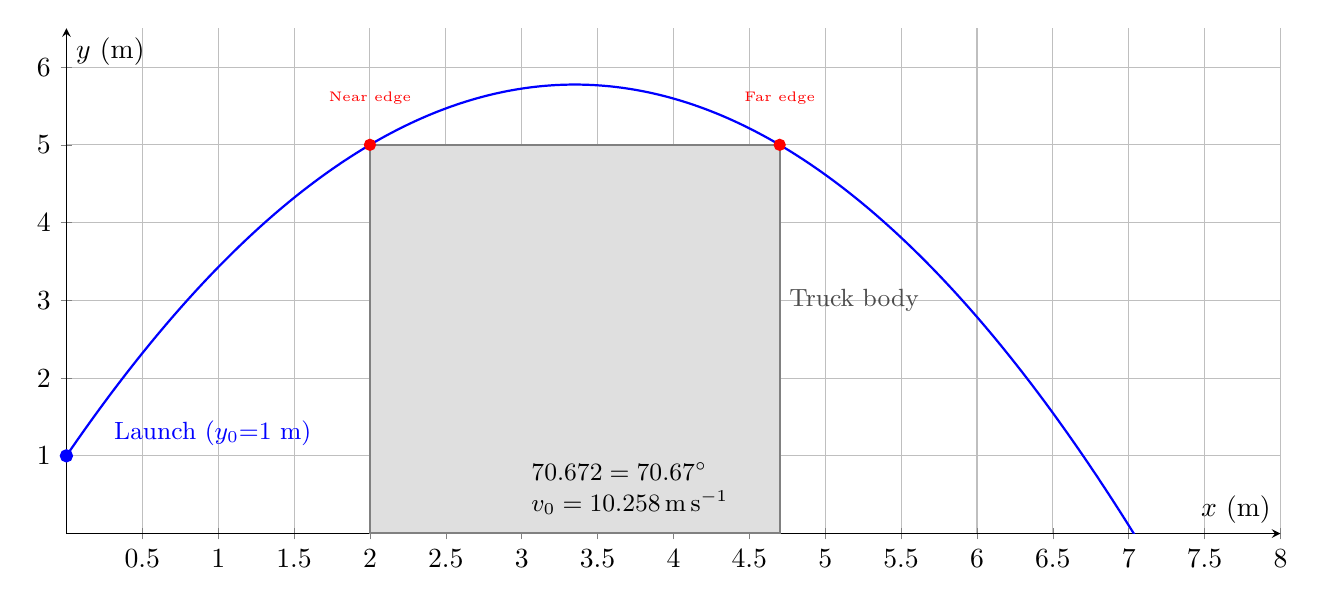
\begin{tikzpicture}
  \begin{axis}[
    width=17cm, height=8cm,
    axis lines=middle,
    xlabel={$x$ (m)}, ylabel={$y$ (m)},
    xmin=0, xmax=8.0,
    ymin=0, ymax=6.5,
    domain=0:10.0,
    samples=400,
    grid=both,
    every axis plot/.append style={thick}
  ]
    % Parameters
    \pgfmathsetmacro{\g}{9.81}   % gravity
    \pgfmathsetmacro{\yzero}{1.0}% launch height
    \pgfmathsetmacro{\D}{2.0}    % standoff to near edge (m)
    \pgfmathsetmacro{\W}{2.7}    % truck width (m)
    \pgfmathsetmacro{\Htop}{5.0} % truck height (m)

    % Optimized launch for D=2.0 m (computed): theta=70.672 deg, v0=10.258 m/s
    \pgfmathsetmacro{\theta}{70.672}
    \pgfmathsetmacro{\vzero}{10.258}
    \pgfmathsetmacro{\thetac}{cos(\theta)}

    % Trajectory: y(x) = y0 + x tanθ - g x^2 /(2 v0^2 cos^2θ)
    \addplot[blue]
      ({x},
       {\yzero + x*tan(\theta) - (\g*x^2)/(2*\vzero*\vzero*\thetac*\thetac)})
      node[pos=0.75, above right] {\small Trajectory};

    % Launch point
    \addplot[only marks, mark=*, mark size=2pt, blue] coordinates {(0,\yzero)};
    \node[anchor=south west, blue] at (axis cs:0.25,\yzero) {\small Launch ($y_0{=}1$ m)};

    % Truck body rectangle [D, D+W] x [0, Htop]
    \addplot[fill=gray!25, draw=gray]
      coordinates {
        (\D,0)
        (\D+\W,0)
        (\D+\W,\Htop)
        (\D,\Htop)
      } -- cycle;

    % Edges and labels
    \draw[dashed, gray] (axis cs:\D,0) -- (axis cs:\D,\Htop);
    \draw[dashed, gray] (axis cs:\D+\W,0) -- (axis cs:\D+\W,\Htop);
    \node[anchor=west, gray!60!black] at (axis cs:\D+\W,3.0) {\small Truck body};

    % Clearance check points at near and far edges
    \addplot[only marks, mark=*, mark size=1.8pt, red]
      coordinates {(\D,\Htop) (\D+\W,\Htop)};
    \node[anchor=south, red] at (axis cs:\D,\Htop+0.4) {\tiny Near edge};
    \node[anchor=south, red] at (axis cs:\D+\W,\Htop+0.4) {\tiny Far edge};

    % Angle and speed annotations
    \node[anchor=west] at (axis cs:3.0,0.8)
      {\small $\theta=\pgfmathprintnumber[fixed,precision=2]{\theta}^\circ$};
    \node[anchor=west] at (axis cs:3.0,0.4)
      {\small $v_{0}=\pgfmathprintnumber[fixed,precision=3]{\vzero}\,\mathrm{m\,s^{-1}}$};
  \end{axis}
\end{tikzpicture}
\caption{Diagram of the trajectory}
\end{figure}

\subsubsection{Assumptions regarding the trajectory}

In order to calculate the trajectory we need to make some assumptions, In this example the standoff distance is 2 metres from the truck body. This is also assuming that the operator is of the average male height and is holding the device roughly 1 metre in the air. Of course this is assuming the worst case scenario being the minimum required velocity.

\subsection{Minimum launch energy}

\subsubsection{Launch energy requirements}

\begin{equation}
    E = \frac{1}{2}mv^2_0 \quad [J]
\end{equation}

\ldots kinetic energy of the launch

\begin{equation}
    J = mv_0 \quad [N \cdot s]
\end{equation}

\ldots specific impulse of the launch

\begin{equation}
    v_{recoil} = \frac{J}{m_{device}+m_{strap}} \quad [m/s]
\end{equation}

\ldots velocity of the recoil produced

\begin{equation}
    F_{peak} \approx \frac{J}{\Delta T} \quad [N]
\end{equation}

\ldots peak force generated by the launch is dependent on the time over which the force damper acts (iterated on in Table \ref{tab:recoil_forces})

\newpage

\subsubsection{Iteration on the masses of the projectiles}


\begin{table}[ht]
\centering
\caption{Projectile energy, impulse and device recoil}
\label{tab:proj_energy_recoil}
\begin{tabular}{@{}rrrrr@{}}
\toprule
Projectile mass $m$ [kg] & $E=\tfrac12 m v_0^2$ [J] & $J=m v_0$ [N$\cdot$ s] & {$v_{\rm rec}=J/m_{\rm}$ [m/s]} & $E_{\rm rec}=\tfrac12 m_{\rm} v_{\rm rec}^2$ [J] \\
\midrule
0.20 & 10.52 & 2.052 & 0.684 & 0.702 \\
0.40 & 21.05 & 4.103 & 1.368 & 2.806 \\
0.60 & 31.57 & 6.155 & 2.052 & 6.314 \\
\bottomrule
\end{tabular}
\begin{tablenotes}[flushleft]
\footnotesize
\textit{Note}. Device mass $(m) = 3kg$.
\end{tablenotes}
\end{table}

\begin{table}[ht]
\centering
\caption{Estimated peak recoil force}
\label{tab:recoil_forces}
\begin{tabular}{@{}rccc@{}}
\toprule
Projectile mass $m$ [kg] & $\Delta$ t=0.05\,$s$ & $\Delta t=0.10$\,$s$ & $\Delta t=0.20$\,$s$ \\
\midrule
0.20 & 41.0 & 20.5 & 10.3 \\
0.40 & 82.1 & 41.0 & 20.5 \\
0.60 & 123.1 & 61.5 & 30.8 \\
\bottomrule
\end{tabular}
\end{table}




\subsubsection{Recoil mitigation requirements}


\newpage

\subsubsection{Launch Energy/Force Sizing}

\subsubsection{Drive Torque and Power Comparison}

\subsection{Estimation of Time Requirements}

\subsection{Calculation of Real-time Requirements}

\subsubsection{Cycle Times by Mode}

\subsubsection{Total Time per Mission}

\newpage

\section{Assembly Drawings}

\newpage

\section{Systems Engineering Management Plan (SEMP)}

\subsection{Scope and Objectives}

\subsection{Roles and Responsibilities}

\subsection{Work Breakdown Structure}

\subsection{Schedule and Milestones}

\subsection{Risk Management}

\subsection{Verification and Validation Plan}

\subsection{Configuration Management}

\subsection{Quality Management}

\subsection{Safety Management}

\subsection{Maintenance and Support Plan}

\newpage

\printbibliography

\newpage

\appendix

\section{FFBDs}

\section{Function Tree}

\section{UR--SR Traceability Matrix}

\section{Interface Definitions}

\section{Test Procedures}

\end{document}

